\documentclass[12pt]{article}

\usepackage[a4paper,margin=2.5cm]{geometry}
\usepackage{amsmath, amssymb, amsthm}
\usepackage{bm}
\usepackage{hyperref}
\usepackage{graphicx}
\usepackage{caption}
\usepackage{listings}
\usepackage{xcolor}
\usepackage{float}
\usepackage{placeins}
\graphicspath{{figures/}}

\lstdefinestyle{code}{
  basicstyle=\ttfamily\small,
  numbers=left,
  numberstyle=\tiny,
  numbersep=8pt,
  keywordstyle=\color{blue},
  commentstyle=\color{teal!70!black},
  stringstyle=\color{orange!70!black},
  showstringspaces=false,
  breaklines=true,
  frame=single,
  framerule=0.3pt,
  rulecolor=\color{black!15}
}
\lstset{style=code}

\title{FP-Growth Association Rule Tutorial}
\author{}
\date{\today}

\begin{document}
\maketitle

\section{Introduction}
The FP-Growth algorithm mines frequent itemsets without candidate generation by compressing transactions into a frequent-pattern tree (FP-tree). After a single database scan builds the FP-tree, recursive conditional mining discovers patterns efficiently, making FP-Growth a popular alternative to Apriori for large and dense datasets.

\section{Theory and Formulas}
\subsection{FP-tree Construction}
Given transactions \(\mathcal{D}\) and a minimum support threshold \(\texttt{min\_supp}\), FP-Growth counts item frequencies, removes infrequent items, and orders each transaction by descending frequency before insertion. Each transaction is mapped into the FP-tree, merging common prefixes and incrementing node counts. A header table maintains links to nodes containing the same item to support traversal.

\subsection{Conditional Pattern Bases}
For each item \(i\) in the header table, FP-Growth gathers all prefix paths ending at \(i\) to form the conditional pattern base. These weighted paths define a conditional FP-tree from which frequent patterns that include \(i\) are mined recursively. The support of an itemset is the sum of counts along paths leading to the item. Because the search explores only frequent prefixes, the algorithm avoids combinatorial explosion.

\subsection{Rule Generation}
Once frequent itemsets are known, association rules \(X \Rightarrow Y\) are derived with the same support, confidence, and lift metrics as Apriori:
\begin{align}
\operatorname{supp}(X) &= \frac{\left|\{ T \mid X \subseteq T,\; T \in \mathcal{D}\}\right|}{|\mathcal{D}|},\\
\operatorname{conf}(X \Rightarrow Y) &= \frac{\operatorname{supp}(X \cup Y)}{\operatorname{supp}(X)},\\
\operatorname{lift}(X \Rightarrow Y) &= \frac{\operatorname{conf}(X \Rightarrow Y)}{\operatorname{supp}(Y)}.
\end{align}
Additional measures such as conviction or leverage help prioritize the most actionable rules.

\section{Applications and Tips}
\begin{itemize}
  \item \textbf{Retail analytics}: identify product bundles and plan promotions in large point-of-sale datasets.
  \item \textbf{Web usage mining}: uncover navigation patterns or co-accessed resources from clickstreams.
  \item \textbf{Industrial monitoring}: detect co-occurring alarms or events in sensor logs.
  \item \textbf{Best practices}: tune \(\texttt{min\_supp}\) to limit tree size, normalize item ordering for deterministic results, limit recursion depth for very dense data, and validate rules against business constraints.
\end{itemize}

\section{Python Practice}
The script \texttt{gen\_fp\_growth\_figures.py} synthesizes transactional data, implements a compact FP-Growth miner, and visualizes the support--confidence distribution and lift histogram for the resulting rules.
\begin{lstlisting}[language=Python,caption={Excerpt from gen_fp_growth_figures.py}]
frequent_itemsets = fpgrowth(transactions, min_support=0.06)
rules = derive_rules(frequent_itemsets, min_confidence=0.5)

for lhs, rhs, support, confidence, lift in rules:
    # store metrics for plotting
    support_vals.append(support)
    confidence_vals.append(confidence)
    lift_vals.append(lift)
\end{lstlisting}

\section{Result}
\begin{figure}[H]
  \centering
  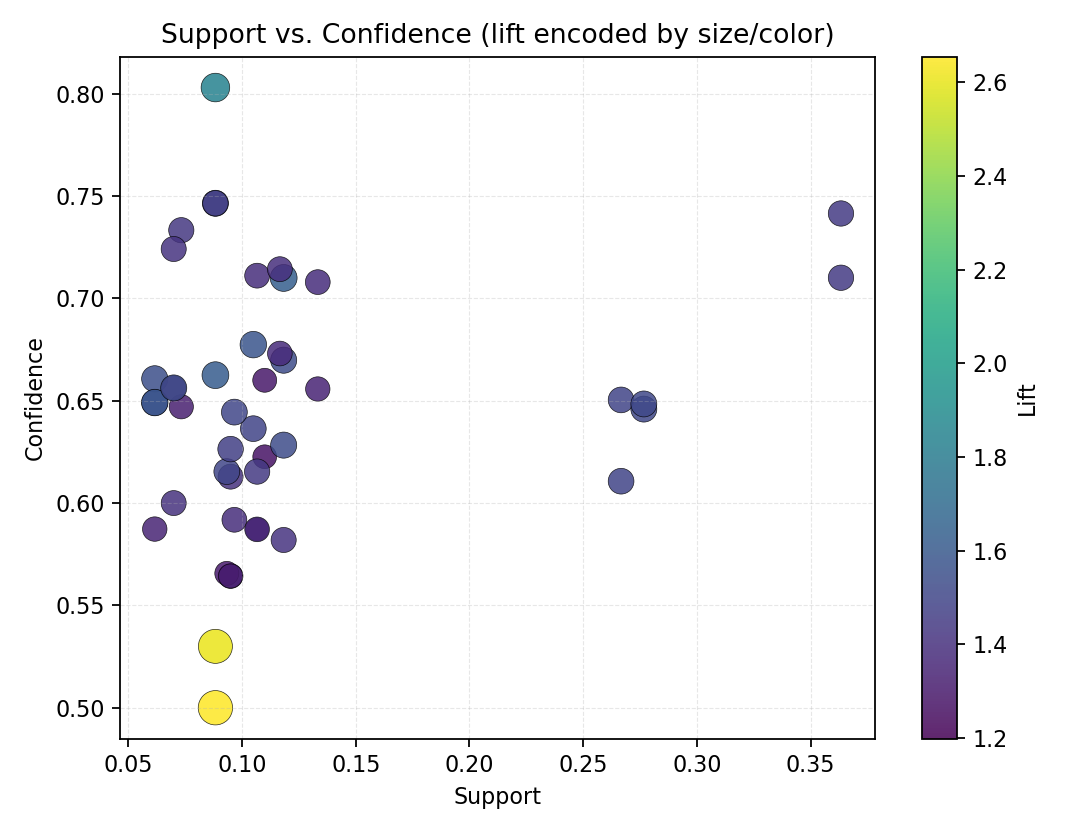
\includegraphics[width=0.82\linewidth]{fpgrowth_support_confidence.png}
  \caption{Support vs. confidence for FP-Growth rules (marker size indicates lift)}
  \label{fig:fpgrowth_support_confidence}
\end{figure}

\begin{figure}[H]
  \centering
  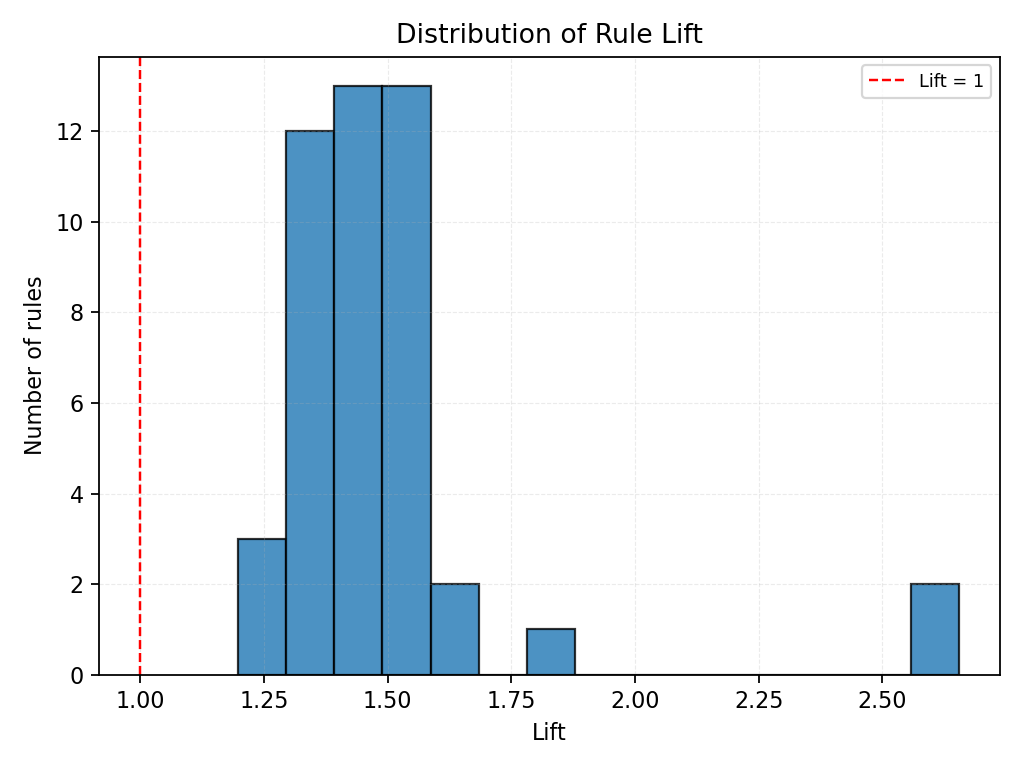
\includegraphics[width=0.78\linewidth]{fpgrowth_lift_distribution.png}
  \caption{Lift distribution highlighting strong associations}
  \label{fig:fpgrowth_lift_distribution}
\end{figure}

\FloatBarrier
\section{Summary}
FP-Growth compresses transactions into an FP-tree and mines frequent patterns without exhaustive candidate generation. By adjusting support thresholds, item ordering, and rule metrics, analysts can extract interpretable association rules even from large datasets. The synthetic example demonstrates how visualization aids in evaluating mined patterns and tuning parameters.

\end{document}
